\graphicspath{ {img/ch0/}, {img/} }

\section*{\textcolor{Blue}{iii. Guía para resolver ejercicios de Ingeniería Económica a partir de la evaluación conceptual}}
\addcontentsline{toc}{section}{iii. Guía para resolver ejercicios de Ingeniería Económica}
\begin{enumerate}
    \item Leer y precisar el enunciado del ejercicio, resaltando las variables independientes, dependientes y los elementos constitutivos para el flujo de caja o diagrama de equivalencia.
    \item Volver a leer para determinar los bloques conceptuales(ejemplo: serie  uniforme proyectada y diferida)
    \item A partir de los bloques determinar primero los subindices de n, luego determinar subindices de valores o series que corresponden a las n.
    \item Estructurar la solución en forma ordenada en 5 pasos: Diagrama de flujo de caja o de equivalencia, declaración de variables, declaración de fórmulas, desarrollo matemático (ECUACIÓN DE VALOR o de equivalencia), respuesta (justificación).
    \textcolor{Blue}{\item \textbf{Construir el diagrama de flujo de caja, mediante:}}
    \begin{itemize}
        \color{Blue}
        \item Un plano cartesiano, para n períodos vencidos o anticipados según el caso y para el actor de referencia (prestamista o prestatario).
        \item El dibujo de los egresos en sentido negativo del eje y, y los ingresos en sentido positivo del eje y.
        \item A la existencia de egresos habrá un ingreso o varios ingresos para poder existir una ecuación de valor.
        \item Una línea horizontal u oblicua que una el flujo final al flujo inicial de la serie uniforme o serie escalonada o gradiente.
        \item Una fecha focal (ff) al final o al comienzo o al intermedio del eje x, que permita visualizar y registrar la ECUACIÓN DE VALOR en el desarrollo matemático.
        \item Los bucles que direccione el sentido positivo (valor futuro) o negativo (valor presente) del valor de equivalencia con respecto a la fecha focal.
        \item Los bucles, en su interior, indicar el n (número de períodos positivos - valor futuro-, negativos - valor presente) a \underline{trasladar a la derecha o izquierda} el componente de la ecuación de valor. Ante la existencia de ``períodos muertos'' en series, gradientes, cambios de tasas u otros, no olvidar ``trasladar'' el VP o VF de la serie, gradiente, etc, a la ff mediante el operador fundamental $P=F(1+i)^{-n}$, según el caso.
        \item La tasa periódica porcentual (i\%) o la tasa periódica anualizada (j\%) de los bucles vencida o anticipada según la modalidad de los períodos. IMPORTANTE: la periodicidad y modalidad de la tasa de interés (i\%) debe ser igual a las de los períodos (n). En su defecto, utilizar la fórmula de conversión de tasas (i\%) y/o de cambio de modalidad (ia\% a i\%).
    \end{itemize}
    \item Declarar las variables, mediante el registro de:
    \begin{itemize}
        \item Las variables independientes, indicando las unidades de cada una, la periodicidad y modalidad de liquidación de intereses y períodos.
        \item La variable o variables dependientes, indicando las unidades y el signo de interrogación.
        \item La verificación de las variables necesarias para la aplicación de las fórmulas.
    \end{itemize}
    \item Declarar las fórmulas, indicando:
    \begin{itemize}
        \item Las fórmulas transitorias y las fundamentales a utilizar, acompañadas del NOMBRE de la misma. 
    \end{itemize}
    \textcolor{Blue}{\item \textbf{Desarrollar el procedimiento matemático, efectuando:}}
    \begin{itemize}
        \color{Blue}
        \item El remplazo matemático de las fórmulas e indicando las unidades correspondientes. 
        \item El registro de la expresión de ECUACIÓN DE VALOR o equivalencia al remplazo matemático correspondiente.
        \item El proceso matemático en forma ordenada, clara y precisa. \\
    \end{itemize}
    \item Registrar la respuesta (justificación), indicando:
    \begin{itemize}
        \item La variable independiente o variables independientes, su respuesta y unidades. \\
    \end{itemize}
\end{enumerate}

\textcolor{Blue}{\textbf{IMPORTANTE 1:}} Volver a leer el enunciado del ejercicio para reconfirmar la respuesta y la justificación. \textbf{\textcolor{ForestGreen}{VALIDAR}} el ejercicio utilizando las fórmulas \textcolor{ForestGreen}{ALGEBRÁICAS} de \textcolor{ForestGreen}{EXCEL}, \textbf{\textcolor{ForestGreen}{FÓRMULAS FINANCIERAS}} de \textcolor{ForestGreen}{EXCEL} y \textbf{\textcolor{ForestGreen}{CRYSTAL BALL}}.\\

\textcolor{Blue}{\textbf{IMPORTANTE 2:}} Aplicar los conceptos de la guía INGECO para articular los formatos y herramientas financieras que requiere fondo emprender en sus convocatorias para financiar planes de negocios como modalidad de grado emprendimiento (Acuerdo 38 de 2015 consejo Académico U Distrital)

\section*{\textcolor{ForestGreen}{iv. Guía para resolver ejercicios de Ingeniería Económica a partir de Excel financiero}}
\addcontentsline{toc}{section}{iv. Guía para resolver ejercicios a partir de Excel financiero}

\begin{enumerate}
    \item Leer y precisar el enunciado del ejercicio, resaltando las variables independientes, dependientes y los elementos constitutivos para el flujo de caja o diagrama de equivalencia. 
    \item Volver a leer para determinar los bloques conceptuales (ejemplo: serie uniforme proyectada y diferida).
    \item A partir de los bloques determinar primero los subíndices de n, luego determinar subíndices de valores o series que corresponden a las n.
    \item Estructurar la solución en forma ordenada en 5 pasos: Declaración de variables, tabla de flujo de caja o tabla de amortización o capitalización de ser necesario, aplicación de fórmulas financieras en Excel, respuesta (justificación) y gráfica.
    \textcolor{ForestGreen}{\item \textbf{Declarar variables mediante el registro de:}}
    \begin{itemize}
        \color{ForestGreen}
        \item Las variables independientes, indicando las unidades de cada una, la periodicidad y modalidad de liquidación de intereses y períodos.
        \item La variable o variables dependientes, indicando las unidades y dejando la celda de estas con un 0.
        \item La verificación de las variables necesarias para la aplicación de la formula.
    \end{itemize}
    \textcolor{ForestGreen}{\item \textbf{Realizar la tabla de flujo de caja de la siguiente forma:}}
    \begin{itemize}
        \color{ForestGreen}
        \item Definir en la columna [1] el número de períodos correspondientes al ejercicio.
        \item En la columna [2] rellenar con el flujo correspondiente a cada período en la columna [1]. 
    \end{itemize}
    \begin{center}
    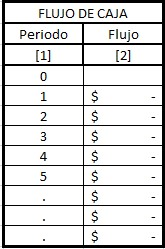
\includegraphics[height=6cm]{0_1}
    \end{center}
    
    En el caso de ser una tabla de amortización se debe rellenar de la siguiente forma: 
    \begin{itemize}
        \color{ForestGreen}
        \item Para todos los valores de [3], [4], [5], [6] en el período 0 se les asignara un valor de \$0.
        \item Definir en la columna [1] el número de períodos correspondientes al ejercicio.
        \item Definir en la columna [2] para el período 1 el valor es igual al rezagado de [6] y arrastrar para todos los períodos.
        \item Definir en la columna [3] para el período 1 el valor de [1] multiplicado por la celda fija en la que se encuentran los intereses y arrastrar para todos los períodos.
        \item Definir en la columna [4] para el período 1 el valor de [5] menos el valor de [6] y arrastrar para todos los períodos.
        \item Definir en la columna [5] el valor de la cuota correspondiente para cada [1] y arrastrar para todos los períodos.
        \item Definir en la columna [6] el valor de [1] menos el valor de [4] y arrastrar para todos los períodos.
    \end{itemize}
    \begin{center}
    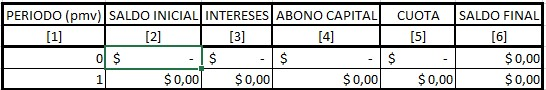
\includegraphics[height=2.35cm]{0_2}
    \end{center}
    
    En el caso de tener una tabla de capitalización de debe rellenar de la siguiente forma:
    \begin{itemize}
        \color{ForestGreen}
        \item Para todos los valores de [1], [2], [3], [4], [5], [6] en el período 0 se les asignara un valor de \$0.
        \item Definir en la columna [1] el número de períodos correspondientes al ejercicio.
        \item Definir en la columna [2] para el período 1 el valor es igual al rezagado de [5] y arrastrar para todos los períodos.
        \item Definir en la columna [3] para el período 1 el valor de la cuota correspondiente para cada [1] y arrastrar para todos los períodos.
        \item Definir en la columna [4] para el período 1 el valor de [2] más el valor [3] multiplicando por la celda fija en la que se encuentran los intereses y arrastrar para todos los períodos.
        \item Definir en la columna [5] para el período 1 la suma de [2], [3] y [4].
    \end{itemize} 
    \begin{center}
    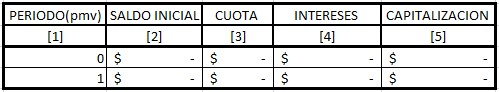
\includegraphics[height=2.5cm]{0_3}
    \end{center}
    \textcolor{ForestGreen}{\textbf{NOTA:} Es una buena idea referenciar todos los valores que se apliquen en el flujo de caja desde la declaración de variables, así al cambiar un valor de la declaración de variables cambiará toda la tabla del flujo de caja y de esta forma se puede aplicar análisis de sensibilidad al ejercicio.} \\ \\ 
    
    \textcolor{ForestGreen}{\item \textbf{Para la aplicación de fórmulas financieras en Excel se deberá tener en cuenta cuál fórmula deberá usarse a partir de las siguientes:}} \\
    

    \begin{enumerate}
    \renewcommand{\labelenumi}{\roman{enumi}}
        \item \textcolor{ForestGreen}{PAGO:} Calcula el pago de un préstamo basado en pagos y tasa de interés constante.
        \begin{center}
        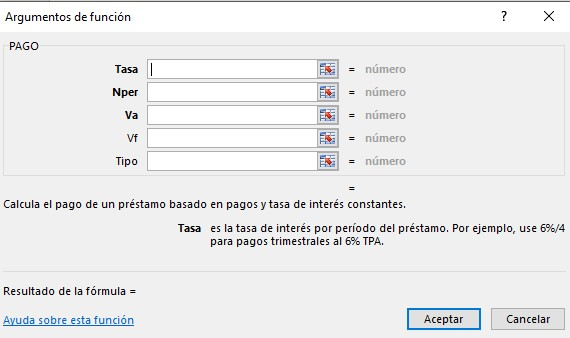
\includegraphics[height=6cm]{0_4} \\
        \end{center}
        \begin{center}
        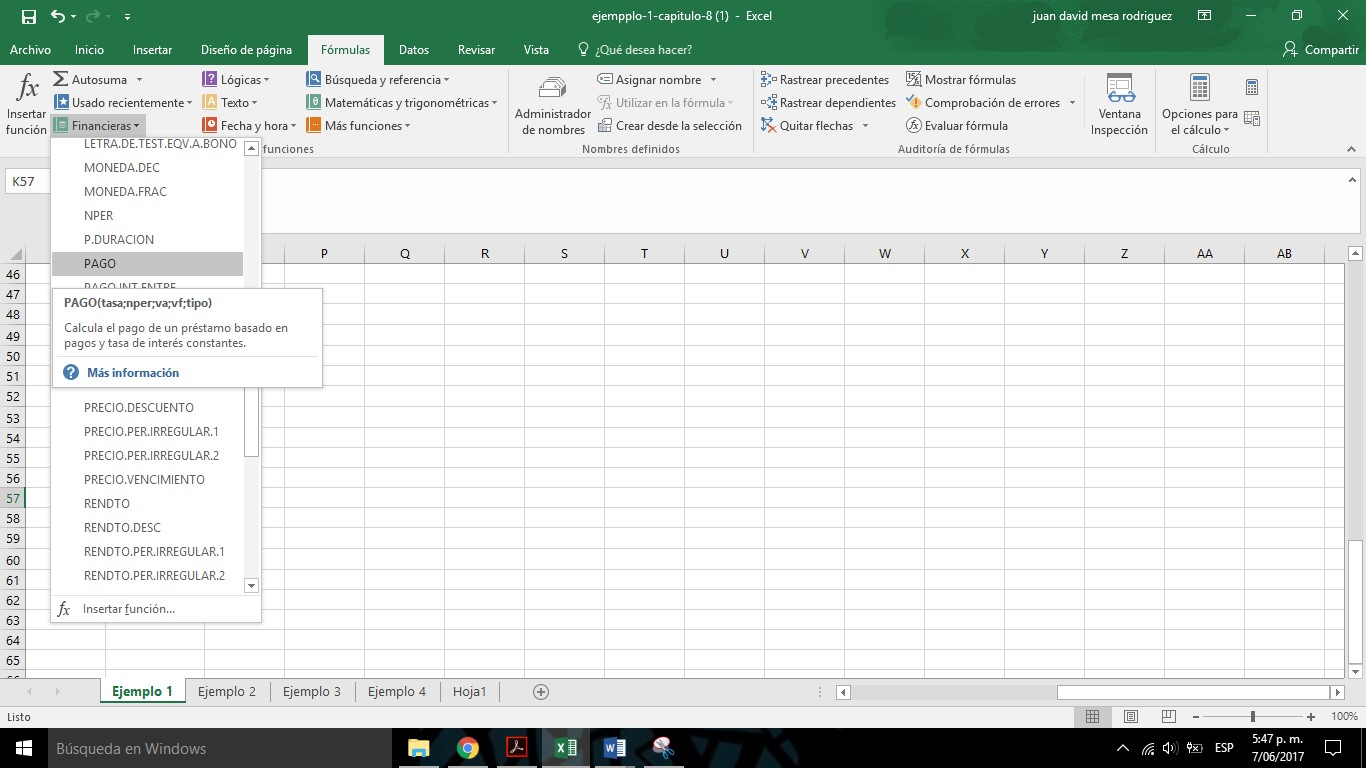
\includegraphics[height=7.41cm]{0_5} 
        \end{center}
        \item \textcolor{ForestGreen}{VA (Valor actual):} Devuelve el valor presente de una inversión; la suma total del valor actual de una serie de pagos futuros.
        \begin{center}
        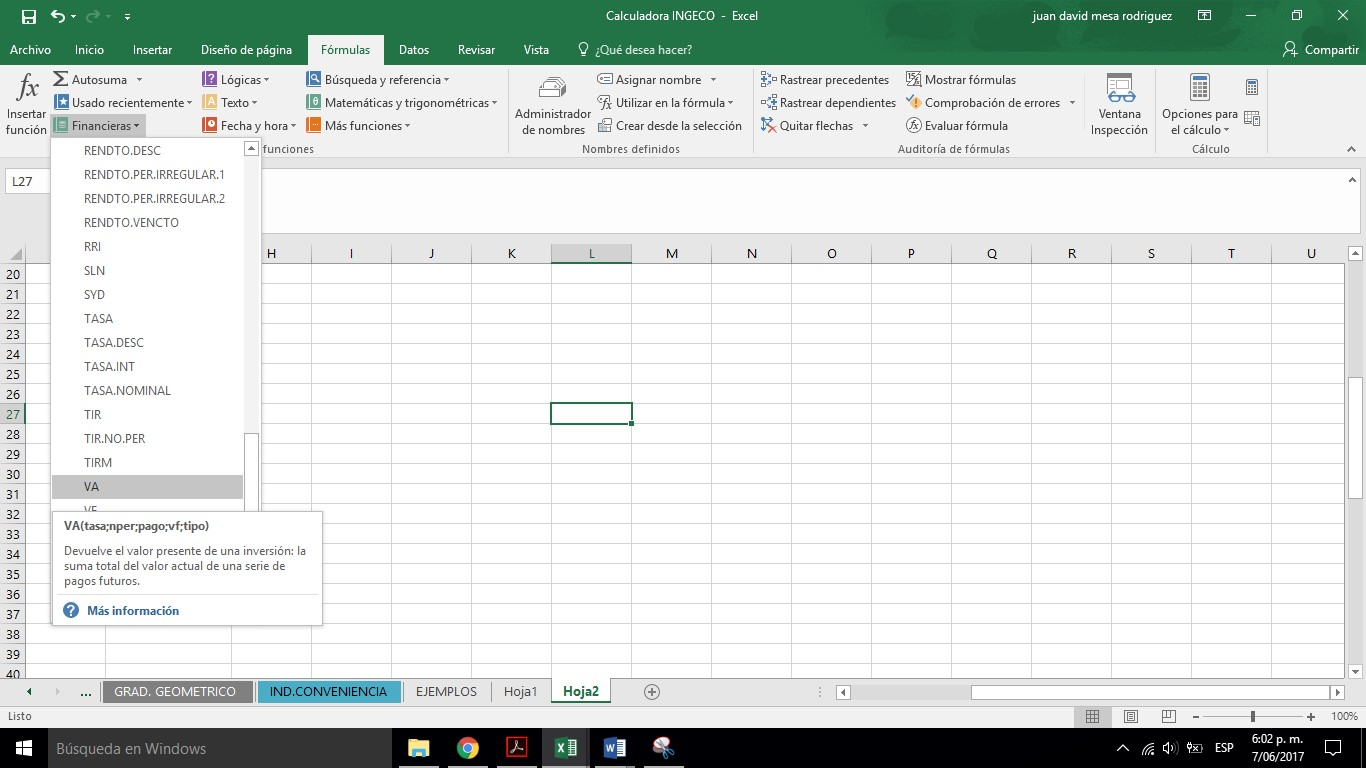
\includegraphics[height=7.41cm]{0_6} \\
        \end{center}
        \begin{center}
        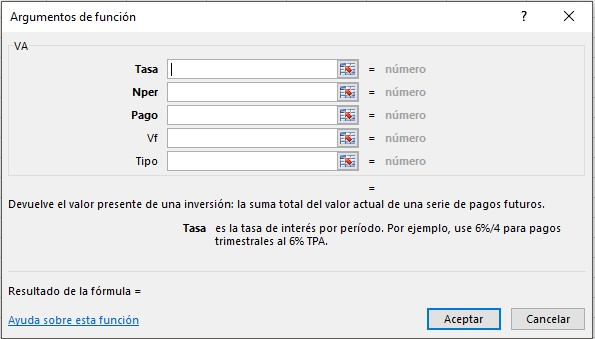
\includegraphics[height=6cm]{0_7}
        \end{center}
        \item \textcolor{ForestGreen}{VF (Valor futuro):} Devuelve el valor futuro de una inversión basado en pagos periódicos y constantes, y una tasa de interés también constante.
        \begin{center}
        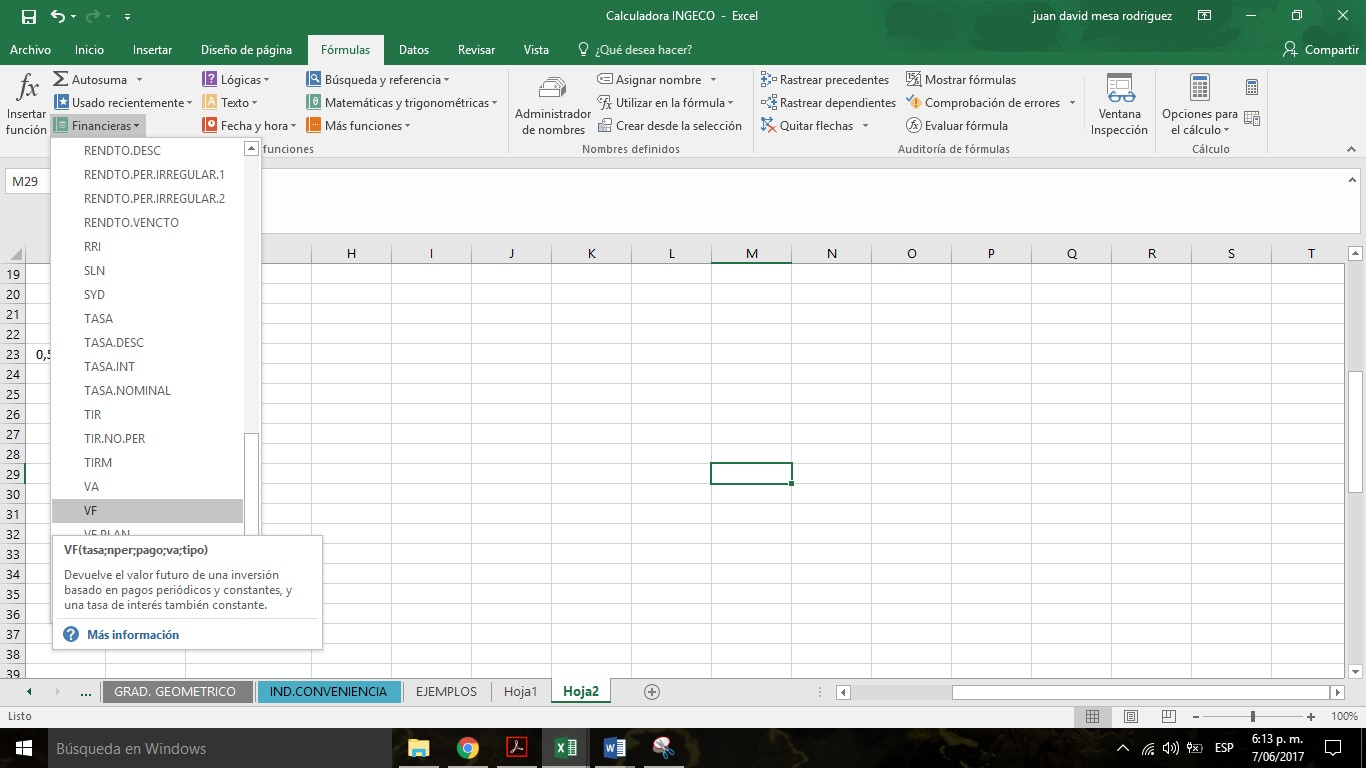
\includegraphics[height=7.15cm]{0_8} \\
        \end{center}
        \begin{center}
        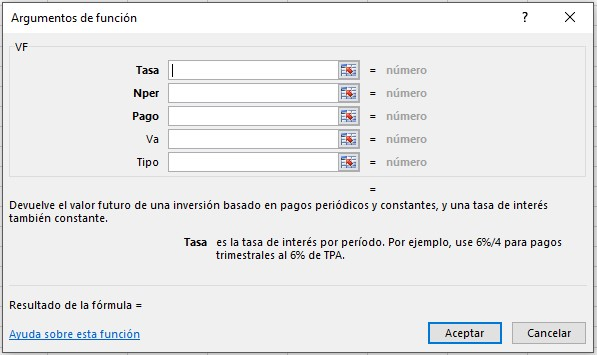
\includegraphics[height=6cm]{0_9}
        \end{center}
        \item \textcolor{ForestGreen}{TASA:} Devuelve el valor de la tasa de interés por período de un préstamo o una inversión.
        \begin{center}
        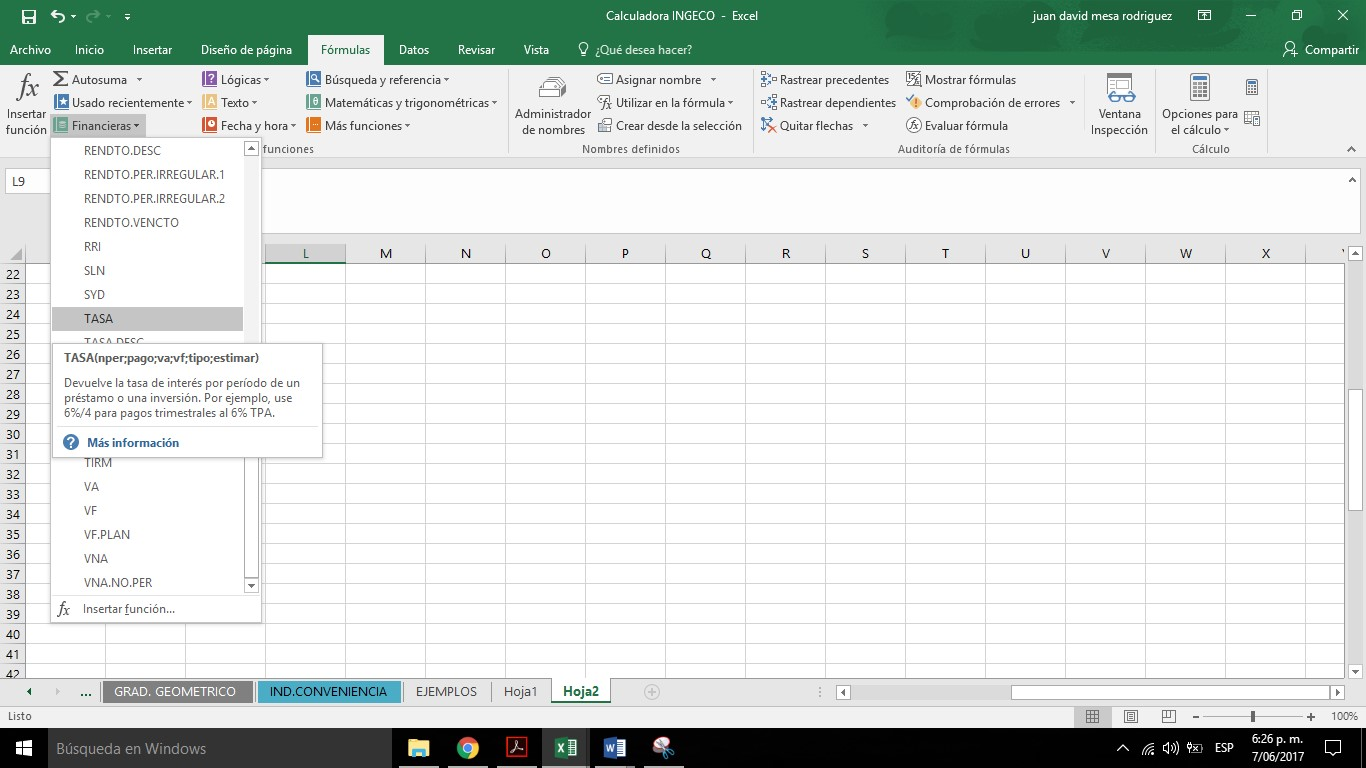
\includegraphics[height=7.15cm]{0_10} \\
        \end{center}
        \begin{center}
        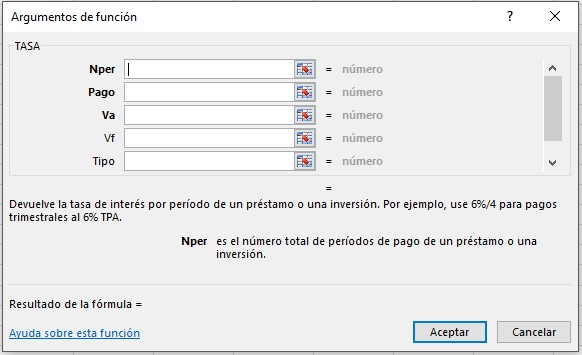
\includegraphics[height=6cm]{0_11}
        \end{center}
        \item \textcolor{ForestGreen}{NPER (Numero de períodos):} Devuelve el número de pagos de una inversión, basado en pagos constantes y periódicos y una tasa de interés constante.
        \begin{center}
        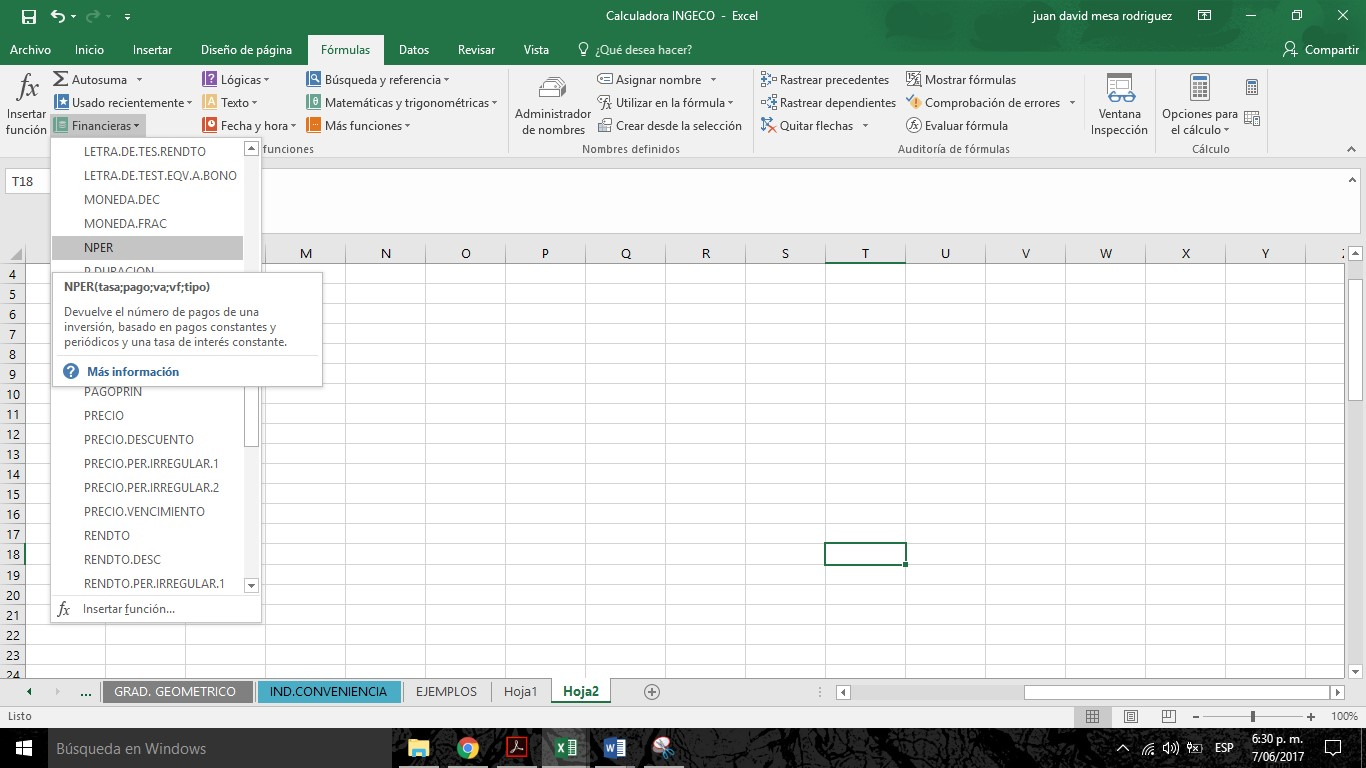
\includegraphics[height=7.15cm]{0_12} \\
        \end{center}
        \begin{center}
        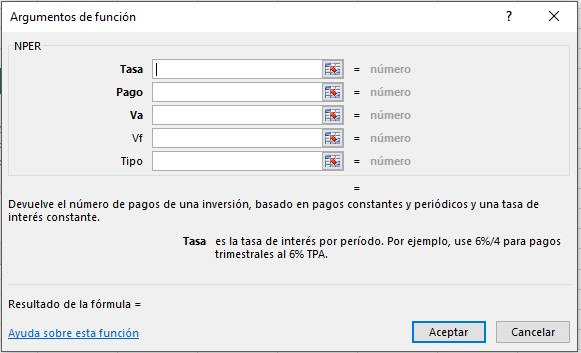
\includegraphics[height=6cm]{0_13}
        \end{center}
        \item \textcolor{ForestGreen}{INT. EFECTIVO (Interés efectivo):} Devuelve la tasa de interés anual efectiva.
        \begin{center}
        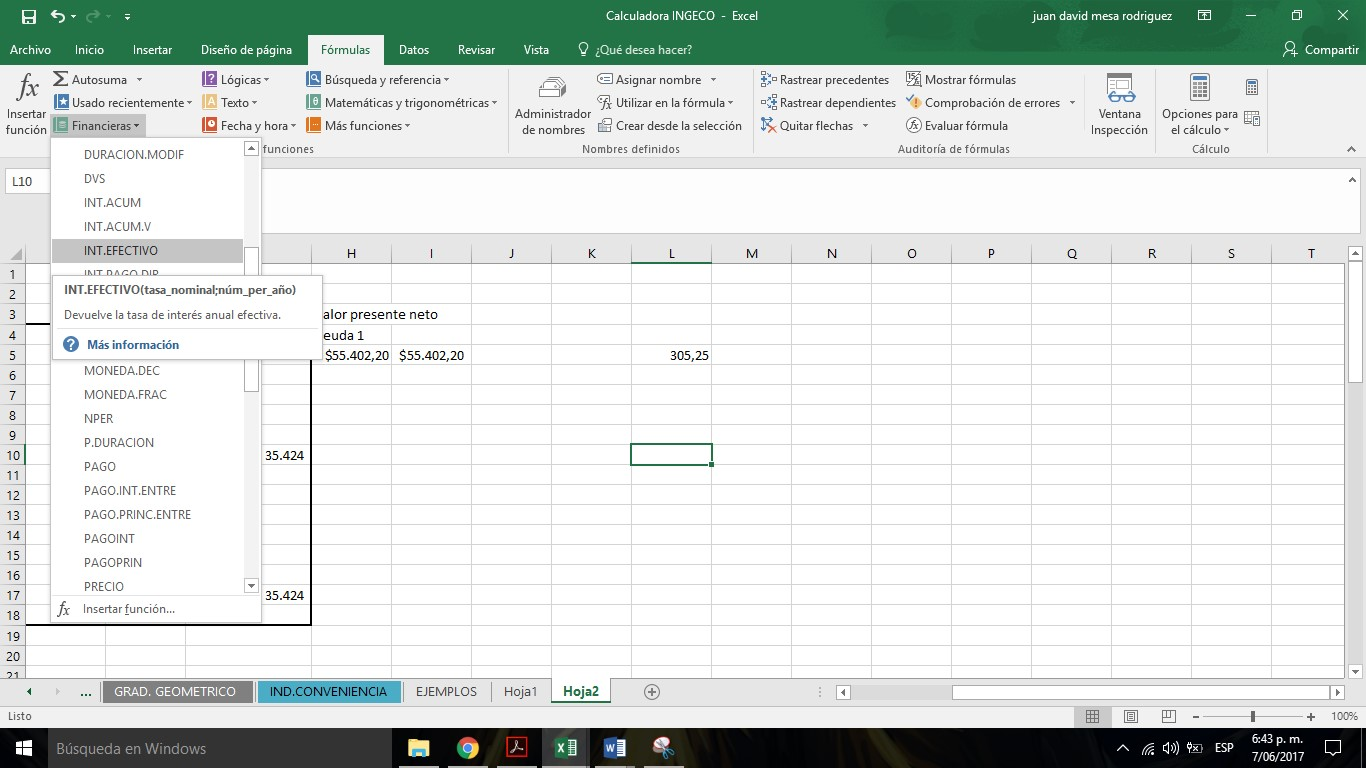
\includegraphics[height=7.15cm]{0_14} \\
        \end{center}
        \begin{center}
        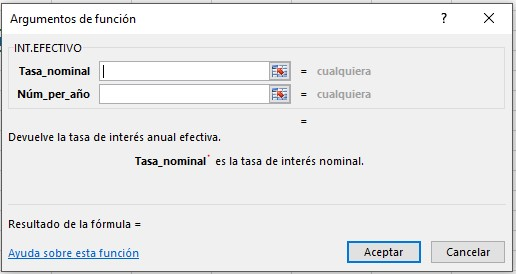
\includegraphics[height=6cm]{0_15}
        \end{center}
        \item \textcolor{ForestGreen}{TASA.NOMINAL:} Devuelve la tasa de interés nominal anual. 
        \begin{center}
        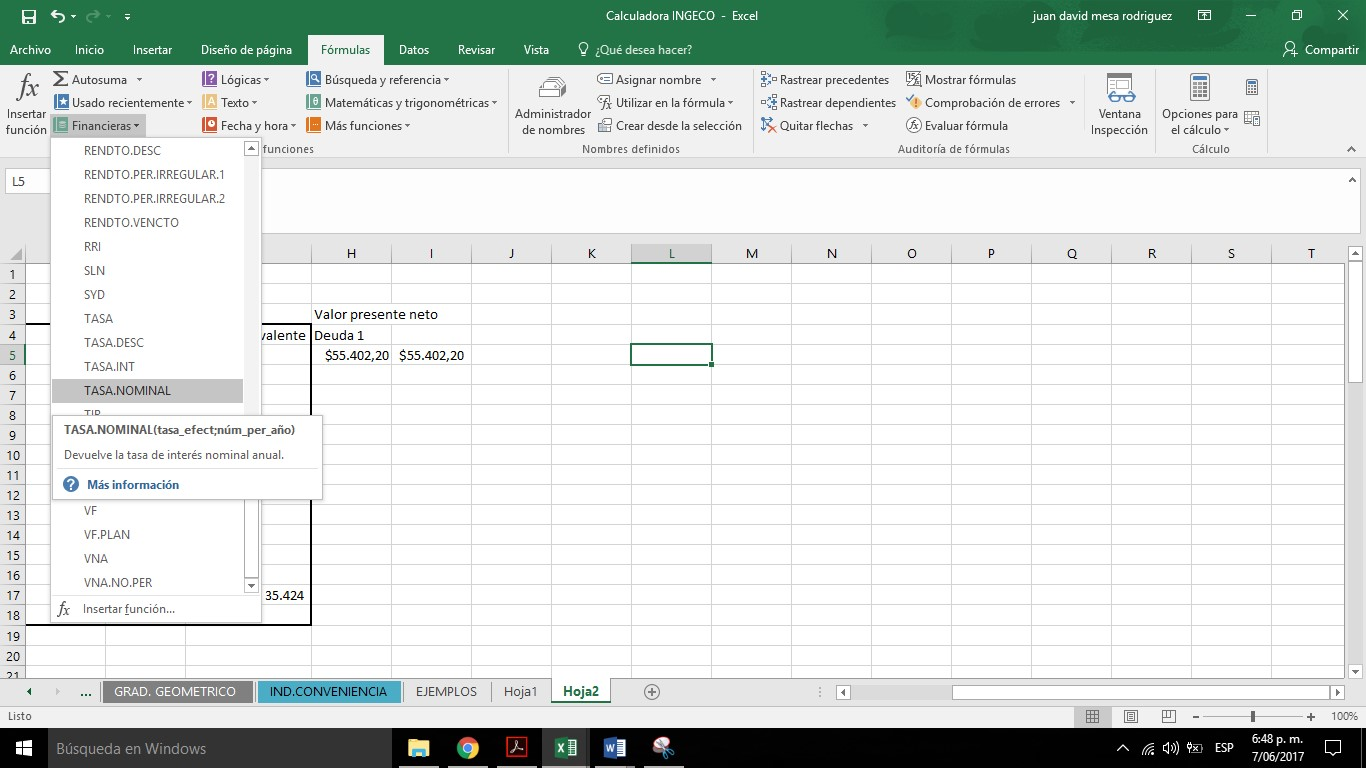
\includegraphics[height=7.15cm]{0_16} \\
        \end{center}
        \begin{center}
        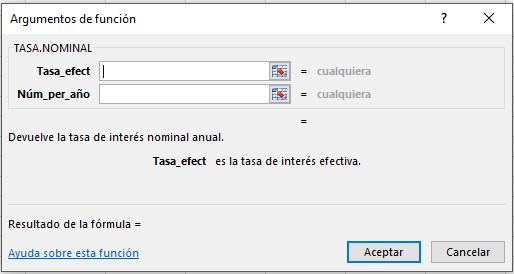
\includegraphics[height=6cm]{0_17}
        \end{center}
        \item \textcolor{ForestGreen}{BUSCAR OBJETIVO:} Encuentra la entrada adecuada para el valor que desee. 
        \begin{center}
        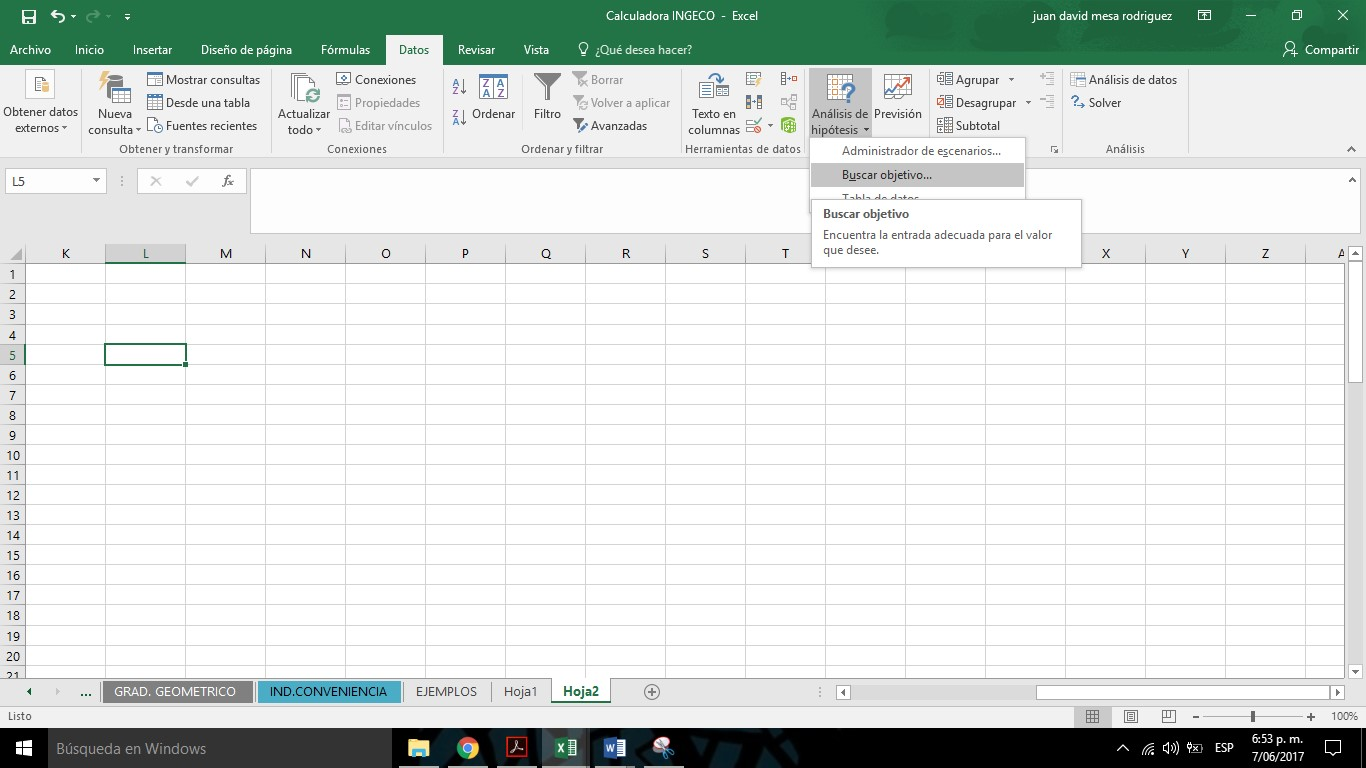
\includegraphics[height=7.15cm]{0_18} \\
        \end{center}
        En la opción de \textcolor{ForestGreen}{“Definir la celda”} se debe colocar la celda sobre la que se encuentra la variable sobre la que se conoce el valor que se desea obtener. \\
        En la opción de \textcolor{ForestGreen}{“Con el valor”} se debe colocar el valor que se desea obtener sobre la variable presente en la opción “Definir la celda”. \\
        En la opción de \textcolor{ForestGreen}{“Cambiando la celda”} se debe colocar la celda que posee la variable que se desea cambiar para llegar al valor que se encuentra en la opción \textcolor{ForestGreen}{“Con el valor”}. \\
        Una vez definidas las opciones Excel realizará los cálculos necesarios y devolverá los valores encontrados sobre las celdas colocadas en la fórmula. \\ \\ 
    
        \begin{center}
        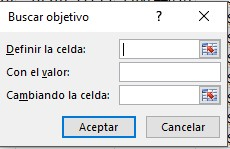
\includegraphics[height=5cm]{0_19}
        \end{center}
    \end{enumerate}
    
    \textcolor{ForestGreen}{\item \textbf{Registrar la respuesta (justificación) indicando:}}
    \begin{itemize}
        \color{ForestGreen}
        \item La variable independiente o variables independientes, su respuesta y unidades.
    \end{itemize}

    \textcolor{ForestGreen}{\item \textbf{Realizar la gráfica correspondiente de la siguiente forma:}}
    \begin{itemize}
        \color{ForestGreen}
        \item La gráfica debe mostrar el comportamiento de los ingresos o egresos a través del número de períodos que posea el problema (Dinero vs Períodos).
        \item Este debe poseer el título del gráfico, los títulos de los ejes y líneas de cuadrícula. 
        \item Se debe especificar las unidades que posee cada eje.
    \end{itemize}


\end{enumerate}


